\chapter{Funzionamento}
Nella seguente sezione si descrive il funzionamento degli stack di guida autonoma e di guida remota del veicolo, degli algoritmi utilizzati e dei nodi realizzati.

\section{Stack di guida autonoma}
La prima cosa che si analizza è il funzionamento dello stack di guida autonoma. Come descritto nel capitolo \ref{introduzione}, questo stack funziona grazie ai processi di perception, planning e control. 

\subsection{Perception} \label{funzionamento_autonomo_perception}
La parte di perception viene implementata avvalendosi delle informazioni del sensore Lidar e mediante la realizzazione dell'algoritmo di localizzazione, concretizzato nei seguenti nodi:
\begin{itemize}
  \item \textbf{urg\_node}: è il nodo che permette di pubblicare sul topic ROS \textit{/scan} le pointcloud rilevate dal sensore Lidar. Il tipo di dato utilizzato è chiamato \textit{LaserScan} e fornisce la serie di distanze rilevate da Lidar.
  
  \item \textbf{hunter\_ros2\_node}: fornisce un'interfaccia con il veicolo, restituendo l'odometria calcolata a partire dal movimento delle ruote e, come vedremo successivamente, permettendo il comando dello stesso. Dal punto di vista della perception, quello che interessa è l'odometria, pubblicata sul topic \textit{/odometry} sottoforma di dato \textit{Odomentry}. 
  
  \item \textbf{particle\_filter}: implementa un algoritmo di localizzazione basato sull'utilizzo di un particle filter e un algoritmo di ray casting. Il suo funzionamento sfrutta la mappa dell'ambiente in cui il robot si sta muovendo, l'odometria del veicolo e la pointcloud del sensore Lidar per il calcolo della posizione. Questo dato viene poi pubblicato sul topic \textit{/pf/position} sottoforma di dato \textit{Odometry}.
\end{itemize}

\begin{figure}[h]
  \centering
  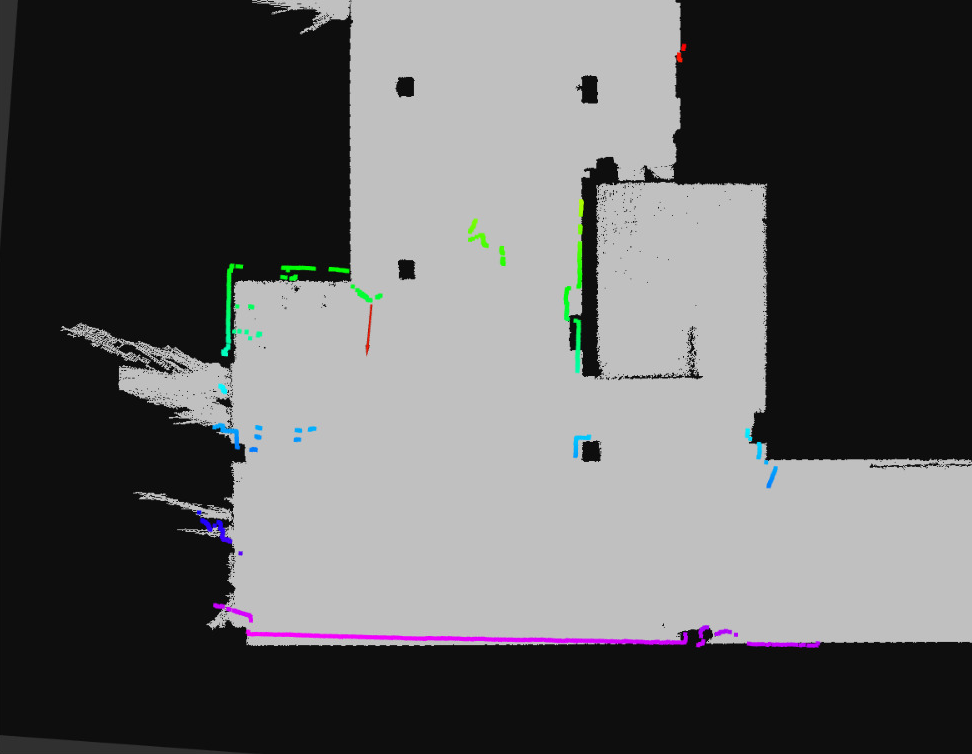
\includegraphics[width=0.7\textwidth]{figures/lidar_map.png}
  \caption{Dimostrazione funzionamento del sensore Lidar}
  \label{funzionamento_particle_filter}
\end{figure}

\noindent Figura \ref{funzionamento_particle_filter} llustra una breve dimostrazione del funzionamento del sensore Lidar. Nello specifico si riporta una porzione di mappa (grigia su sfondo nero) e la pointcloud generata dal sensore Lidar (punti colorati). Il colore dei punti non è casuale, ma è bensì un metodo intuitivo per mostrare graficamente la distanza di quel particolare punto dalla posizione calcolata del robot (freccia rossa).

\subsection{Planning}
\noindent La parte di planning si avvale di due nodi:

\begin{itemize}
  \item \textbf{path\_logger}: permette la registrazione di un percorso quando il veicolo viene guidato manualmente. Il percorso registrato viene poi salvato in un file apposito.
  \item \textbf{path\_publisher}: questo nodo si occupa di pubblicare un percorso preregistrato o precalcolato da seguire, pubblicato sul topic \textit{/path}.  
\end{itemize}

\subsection{Control}
\noindent Si passa infine a descrivere il funzionamento della parte di controllo, composta anch'essa da due nodi:

\begin{itemize}
  \item \textbf{purepursuit}: si occupa di ricevere il percorso pubblicato sul topic \textit{/path} e, a partire dalla posizione pubblicata dal nodo \textbf{particle\_filter}, di calcolare i comandi da impartire al veicolo. I comandi vengono pubblicati sul topic \textit{/drive\_parameters} e sono di tipo \textit{Ackermann Stamped}, un tipo di messaggio ROS che incapsula il timestamp, l'angolo di sterzo e la velocità desiderata
  \item \textbf{hunter\_ros2\_node}: come descritto in precedenza, questo nodo, oltre a fornire l'odometria del mezzo, è anche capace di ricevere i comandi da impartire al veicolo. Il nodo è infatti in perenne ascolto sul topic \textit{/drive\_parameters} e ad ogni messaggio comunicherà con l'interfaccia CAN del veicolo impartendogli la velocità e l'angolo di sterzo desiderati
\end{itemize}

\noindent Di seguito uno schema riassuntivo del funzionamento della guida autonoma:
\begin{figure}[h]
  \centering
  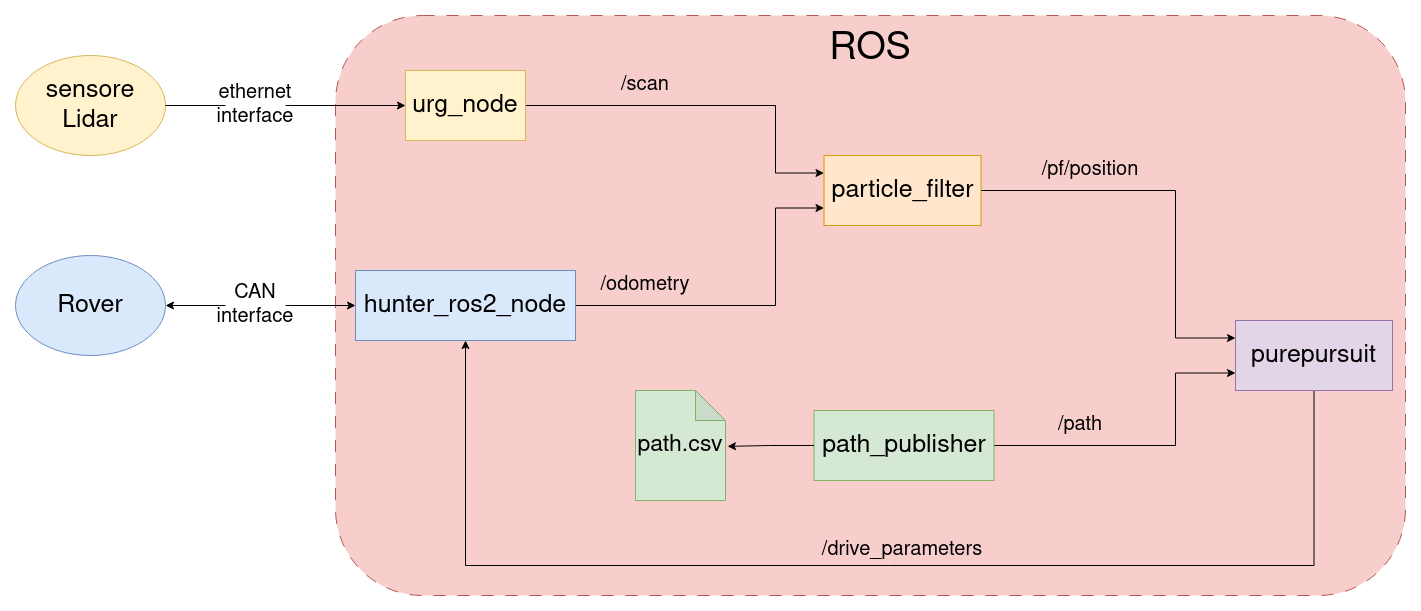
\includegraphics[width=1\textwidth]{figures/schema_guida_autonoma.png}
  \caption{Schema rissuntivo dello stack di guida autonoma}
  \label{Schema rissuntivo dello stack di guida autonoma}
\end{figure}

\section{Guida remota}
Una volta illustrato e compreso il funzionamento dello stack di guida autonoma, si passa alla descrizione di quella remota.

\noindent La prima scelta tecnica è stata quella di decidere quale parte dello stack spostare in remoto. Per esempio, si potrebbe decidere di svolgere solo la parte di planning da remoto e lasciare in resto in locale, o diversamente, portare sin remoto solo la perception. Si potrebbe anche decidere di far eseguire solo specifici nodi da remoto e lasciare in resto in locale.

\noindent Nella presente tesi si è scelto di portare in remoto quasi tutto lo stack, lasciando in locale solo i nodi che hanno strettamente bisogno dell'interfacciamento con l'hardware.

\noindent Nello specifico, gli unici nodi che rimarranno in locale saranno:

\begin{itemize}
  \item \textbf{urg\_node}: che sarà necessario per ricavare i dati dal sensore Lidar
  \item \textbf{hunter\_ros2\_node}: necessario per ricavare l'odometria del mezzo e per inviare i comandi all'interfaccia CAN
\end{itemize}

\noindent Tutto il resto sarà gestito da remoto. Questo permette di poter scegliere con più flessibilità in quale modo pilotare il rover. Si potrà infatti decidere sia di eseguire l'intero stack, senza modifiche, sulla macchina in remoto e di conseguenza inviare i comandi calcolati al mezzo, sia di poter guidare il veicolo completamente in manuale da un apposito operatore e di inviare solo i comandi scelti da quest'ultimo al veicolo.

\noindent Di seguito uno schema riassuntivo del funzionamento della guida remota:

\begin{figure}[h]
  \centering
  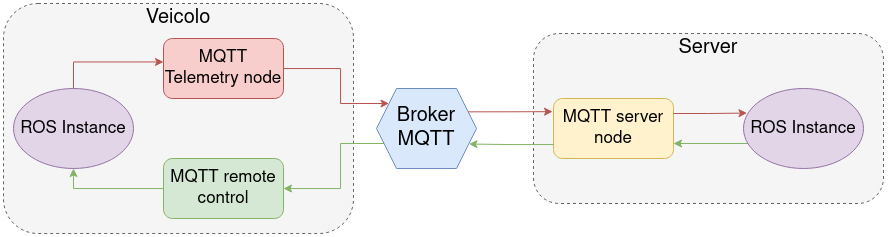
\includegraphics[width=1\textwidth]{figures/schema_guida_remota.png}
  \caption{Schema rissuntivo dello stack di guida remota}
  \label{Schema rissuntivo dello stack di guida remota}
\end{figure}

\section{Nodi sviluppati}
Oltre ai nodi già compresi nello stack di guida autonoma, è stato necessario sviluppare i nodi che permettessero lo scambio di informazioni tra il veicolo e il server. Nello specifico, i 3 nodi sono:
\begin{itemize}
    \item \textbf{mqtt\_telemetry\_node}: ha il compito di inviare i dati dei sensori dal veicolo al server
    \item \textbf{mqtt\_control\_node}: ha il compito di ricevere i dati di controllo dal server per poi pubblicarli su ROS
    \item \textbf{mqtt\_server\_node}: eseguito sul server, avrà il compito di ricevere sia i dati di telemetria da MQTT per poi ripubblicarli su ROS che ricevere i dati di controllo da ROS per poi ripubblicarli su MQTT
\end{itemize}

\noindent Ogni nodo è diviso in più classi ed un unico main file, che gestirà l'intero flusso di esecuzione del nodo. All'interno del progetto che contiene il nodo sono anche compresi dei file di configurazione in formato yaml, dai quali il nodo andrà a leggere informazioni necessarie per l'esecuzione del processo. Di seguito un esempio di file di configurazione utilizzato per definire alcuni parametri relativi alla comunicazione MQTT.

\lstinputlisting{samples/mqtt_parameters.yaml}

\noindent È inoltre utile specificare che l'intera codebase è scritta in linguaggio C++, che risulta utile qualora sia necessario avere bassi tempi di esecuzione.

\subsection{MQTT telemery node} \label{mqtt_telemetry_node}
La prima fase del progetto ha riguardato lo sviluppo di un componente software, ovvero un nodo ROS, in grado di interfacciarsi con i sensori del veicolo. Questo nodo, una volta configurato per sottoscriversi ai topic di interesse, è in grado di acquisire i dati provenienti dai sensori e di trasformarli in un formato adatto alla trasmissione. La scelta del formato JSON, ampiamente utilizzato per lo scambio di dati tra sistemi eterogenei, è stata dettata dalla sua leggibilità e dalla sua facilità di parsing. I dati, una volta formattati, vengono inviati al server MQTT.

\noindent I topic a cui il nodo effettua una subscribe sono:

\begin{itemize}
  \item \textit{/scan}: per la ricezione della pointcloud rilevata dal sensore Lidar
  \item \textit{/odometry}: per la ricezione dei dati di odometria del mezzo
\end{itemize}

\noindent Una volta acquisito il dato grezzo, esso viene convertito in una rappresentazione strutturata e leggibile, che nello specifico si compone di una stringa in formato JSON. Tale stringa, contenente l'insieme completo dei dati costituenti il messaggio, viene quindi immessa all'interno di una cache dedicata.

\noindent La cache funge da deposito temporaneo, accumulando le stringhe JSON generate fino al raggiungimento di una determinata soglia (o intervallo) di tempo predefinito e impostabile tramite file di configurazione. Al verificarsi di tali condizioni, il contenuto completo della cache viene trasmesso in un'unica operazione al server MQTT. Questa modalità di trasmissione, basata su un meccanismo di invio periodico, consente di ottimizzare le comunicazioni e ridurre il carico sulla rete.

\noindent Per quanto concerne la gestione concorrente di queste operazioni, si introduce il concetto di thread. Un thread può essere definito come un flusso di esecuzione autonomo all'interno di un processo. In altre parole, rappresenta una singola sequenza di istruzioni che può essere eseguita in parallelo rispetto ad altre sequenze, all'interno dello stesso programma.

\noindent Nel contesto descritto, è possibile impiegare un thread dedicato per gestire l'operazione di trasmissione dei dati. Tale thread opererà in modo concorrente rispetto al thread principale (main thread) consentendo di eseguire contemporaneamente altre attività e di migliorare la reattività dell'applicazione. Per fare questo è però necessario gestire la cache in modo che i 2 thread che ne fanno utilizzo non vadano in conflitto per accedere alla risorsa in quanto, se ciò non fosse gestito, si andrebbe ad incappare in problemi come, ad esempio, la lettura di un dato incorretto da parte del thread di invio dei messaggi o una scrittura parziale da parte del main thread.

\noindent Per la gestione di questi eventi si è dunque deciso di utilizzare una struttura chiamata mutex, che permette ad un thread di bloccare una risorsa per utilizzarla ed ad un altro di aspettare che la risorsa si liberi per poterla utilizzare. Di seguito l'implementazione della classe \textbf{msgs\_cache}:

\lstinputlisting{samples/msgs_cache.cpp}

\noindent Il nodo è suddiviso in 6 classi:

\begin{itemize}
  \item \textbf{conf\_loader}: si occupa di caricare i dati dai file di configurazione prima citati. Nello specifico, questa classe è stata implementata per rendere il main thread e il resto del processo indipendente dal formato dei file di configurazione
  \item \textbf{mqtt\_publisher}: è una classe che contiene metodi utili all'invio di stringhe tramite protocollo MQTT, avvalendosi della libreria paho.mqtt.cpp fornita dalla eclipse foundation 
  \item \textbf{mqtt\_telemetry\_node}: questa classe è quella che implementa il nodo ROS che si incaricherà di ricevere i dati utili alla telemetria
  \item \textbf{msgs\_cache}: questa classe implementa una semplice struttura dati che accoppia ad ogni topic ROS (rappresentata come stringa), una stringa JSON contente i dati di telemetria da inviare
  \item \textbf{msgs\_to\_string}: è un insieme di funzioni statiche che permette la traduzione da messaggi ROS a stringhe JSON
  \item \textbf{topic\_manager}: è la classe designata ad accoppiare i topic ROS con i rispettivi topic MQTT, il cui codice è incluso nella sezione \ref{gestione_dei_topic} 
\end{itemize}

\subsection{MQTT remote control} \label{mqtt_remote_control}
Successivamente, è fondamentale predisporre un meccanismo che consenta al veicolo di ricevere i comandi di controllo. A tal fine, è stato implementato un nodo dedicato che si sottoscrive al topic MQTT specificamente designato per la trasmissione di tali dati. Successivamente, il nodo ripubblica le informazioni ricevute sul topic ROS \textit{/drive\_parameters}.

\noindent Poiché i dati trasmessi tramite MQTT sono di tipo stringa, il veicolo dovrà elaborare queste stringhe al fine di estrarre le informazioni pertinenti e popolarne i campi di un messaggio ROS conforme al tipo di dato previsto, esattamente come descritto nella sezione 4.3.

\noindent il nodo in questo caso è suddiviso in 4 classi: 

\begin{itemize}
  \item \textbf{conf\_loader}: il cui funzionamento è riportato nella sezione \ref{mqtt_telemetry_node}
  \item \textbf{control\_node}: è il nodo incaricato di ripubblicare sul topic giusto i dati relativi al controllo
  \item \textbf{json\_to\_ros2\_msgs}: è il nodo incaricato alla conversione dei messaggi
  \item \textbf{mqtt\_subscriber}: è il nodo che si occupa alla sottoscrizione al topic mqtt designato alla ricezione dei dati
\end{itemize}

\noindent In questo caso non è stato necessario l'utilizzo della classe \textbf{topic\_manager} in quanto gli unici due topic in gioco (quello ROS e quello MQTT) sono entrambe impostabili da file di configurazione yaml.

\subsection{MQTT server node}
È stato infine implementato un nodo centrale, eseguito sul server, che funge da ponte di comunicazione tra il veicolo e l'istanza ROS del server stesso. Questo nodo è responsabile della ricezione di tutti i dati trasmessi dal veicolo tramite il protocollo MQTT e della loro successiva pubblicazione sul bus ROS. Contestualmente, il nodo si occupa di raccogliere i comandi di controllo generati all'interno dell'ambiente ROS, di incapsularli in un messaggio MQTT e di inoltrarlo al veicolo.

\noindent Il nodo in questo caso è suddiviso in 8 classi, alcune delle quali sono prese dai due nodi prima implementati:

%COSÌ FA CAFARE. SCRIVI ALMENO CHE TALE CLASSE È DESCRITTA IN TAL CAPITOLO, NON LASCIARE L'ELECON VUOTO
\begin{itemize}
  \item \textbf{conf\_loader}: il cui compito è riportato nella sezione \ref{mqtt_telemetry_node}
  \item \textbf{mqtt\_publisher}: il cui compito è riportato nella sezione \ref{mqtt_telemetry_node}
  \item \textbf{mqtt\_subscriber}: descritto nella sezione \ref{mqtt_remote_control}
  \item \textbf{msgs\_cache}: anch'esso descritto alla sezione \ref{mqtt_telemetry_node}
  \item \textbf{msgs\_to\_string}: riportato alla sezione \ref{mqtt_telemetry_node}
  \item \textbf{ros\_server\_node}: implementa il client ROS che andrà poi ad iscriversi e a pubblicare sui topic necessari
  \item \textbf{string\_to\_msgs}: al contrario di \textbf{msgs\_to\_string}, questa classe è incaricata di convertire le stringhe in formato JSON in messaggi ROS
  \item \textbf{topic\_manager}: già riportato alla sezione \ref{mqtt_telemetry_node}
\end{itemize}

\section{Gestione dei topic} \label{gestione_dei_topic}
Come descritto nella sezione \ref{mqtt_topic}, i topic ROS utilizzati hanno una struttura sostanzialmente diversa da quelli MQTT. Ai fini del progetto è stata dunque sviluppata una classe chiamata \textit{topic\_manager} che semplifica la gestione di questi due tipi di dati. La classe comprende 4 semplici metodi, 2 che riguardano il get ed il set di topic ROS e 2 che riguardano il get e il set dei topic MQTT, ad ogni topic MQTT è associato uno ROS e viceversa, di seguito i 4 metodi:

\lstinputlisting{samples/topic_manager.cpp}